\begin{figure}
  \centering
  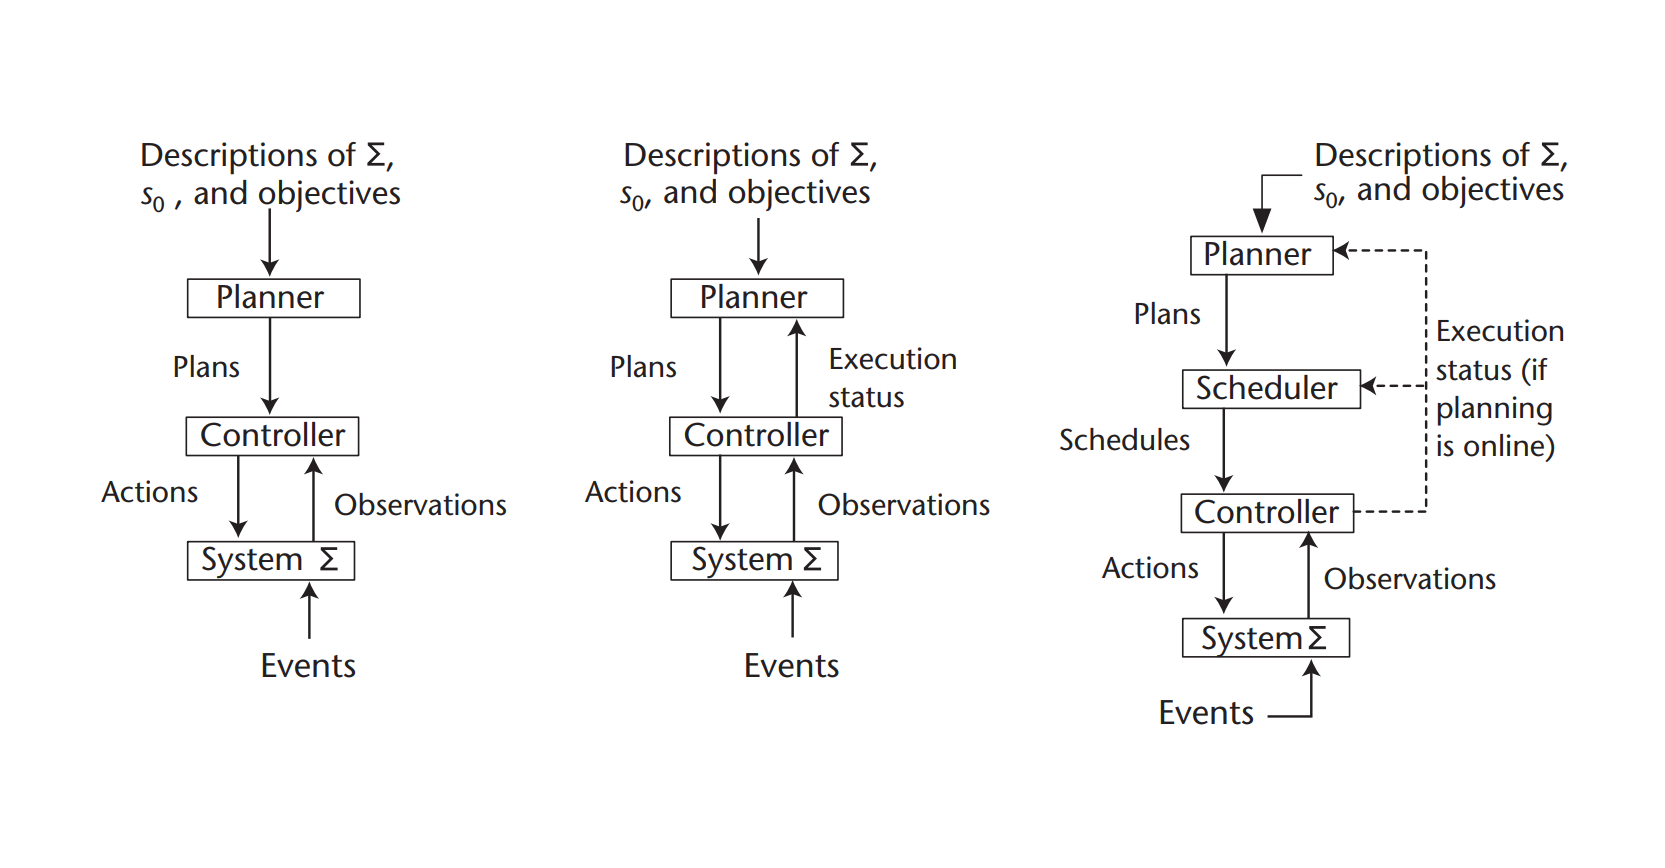
\includegraphics[width=1\linewidth]{figures/planner-diagram.png}
  \caption{Simple Conceptual Models for (a) Offline Planning, (b) Online
    Planning, and (c) Planning with a Separate Scheduler.}
  \label{fig:planner-diagram}
\end{figure}

\newenvironment{sspara}
  {\begin{quote}
    \sffamily
  }
  {
    \normalfont
   \end{quote}
  }

This chapter has been included in verbatim from \cite{Nau2007}'s work describing
the current trends in automated planning. It is included to help give context to
the assumptions at the end of this section which I have used as examples of
restrictions to the planning model. In his work \cite{Nau2007} describes a
conceptual model for planning as the following:

\section{Conceptual Model for Planning}
A conceptual model is a simple theoretical device for describing the main
elements of a problem. It may fail to address several of the practical details
but still can be very useful for getting a basic understanding of the problem.
In this article, I'll use a conceptual model for planning that includes three
primary parts (see figure \ref{fig:planner-diagram}a and
\ref{fig:planner-diagram}b), which are discussed in the following sections: a
\textit{state-transition system}, which is a formal model of the real-world
system for which we want to create plans; a \textit{controller}, which performs
actions that change the state of the system; and a \textit{planner}, which
produces the plans or policies that drive the controller.

\section{State-Transition Systems}
Formally, a \textit{state-transition system} (also called a
\textit{discrete-event system}) as a 4-tuple $\sum = (S, A, E, \gamma)$, where

\begin{sspara}
$S=\{s_0, s_1, s_2, ...\}$ is a set of states;

$A=\{a_1, a_2, ...\}$ is a set of \textit{actions}, that is, state transitions
whose occurrence is controlled by the plan executor;

$E=\{e_1, e_2, ...\}$ is a set of \textit{events}, that is, state transitions
whose occurrence is not controlled by the plan executor;

$\gamma:S \times (A \cup E) \rightarrow 2^S$ is a state-transition function;
\end{sspara}

A state-transition system may be represented by a directed graph whose nodes are
the states in $S$. If $s' \in \gamma (s, e)$, where $e \in A \cup E$ is an
action or event, then the graph contains a \textit{state transition} (that is,
an arc) from $s$ to $s'$ that is labeled with the action or event $e$.

\begin{sspara}
  If $a$ is an action and $\gamma(s, a)$ is not empty, then action $a$ is
  \textit{applicable} to state $s$: if the plan executor executes $a$ in state
  $s$, this will take the system to some state in $\gamma(s, a)$.

  If $e$ is an event and $\gamma(s, e)$ is not empty, then $e$ may $possibly$
  occur when the system is in state $s$. This event corresponds to the internal
  dynamics of the system, and cannot be chosen or triggered by the plan
  executor. Its occurrence in state $s$ will bring the system to some state in
  $\gamma(s, e)$.
\end{sspara}

Given a state-transition system $\sum$, the purpose of planning is to find which
actions to apply to which states in order to achieve some objective, when
starting from some given situation. A \textit{plan} is a structure that gives
the appropriate actions. The objective can be specified in several different
ways. The simplest specification consists of a \textit{goal state} $s_g$ or a
set of goal states $S_g$ . For example, if the objective in figure
\ref{fig:state-transition-diagram} is to have the container loaded onto the
robot cart, then the set of goal states is $S_g = \{s_4, s_5\}$. In this case, the
objective is achieved by any sequence of state transitions that ends at one of
the goal states. More generally, the objective might be to get the system into
certain states, to keep the system away from certain other states, to optimize
some utility function, or to perform some collection of tasks.

\begin{figure}
  \centering
  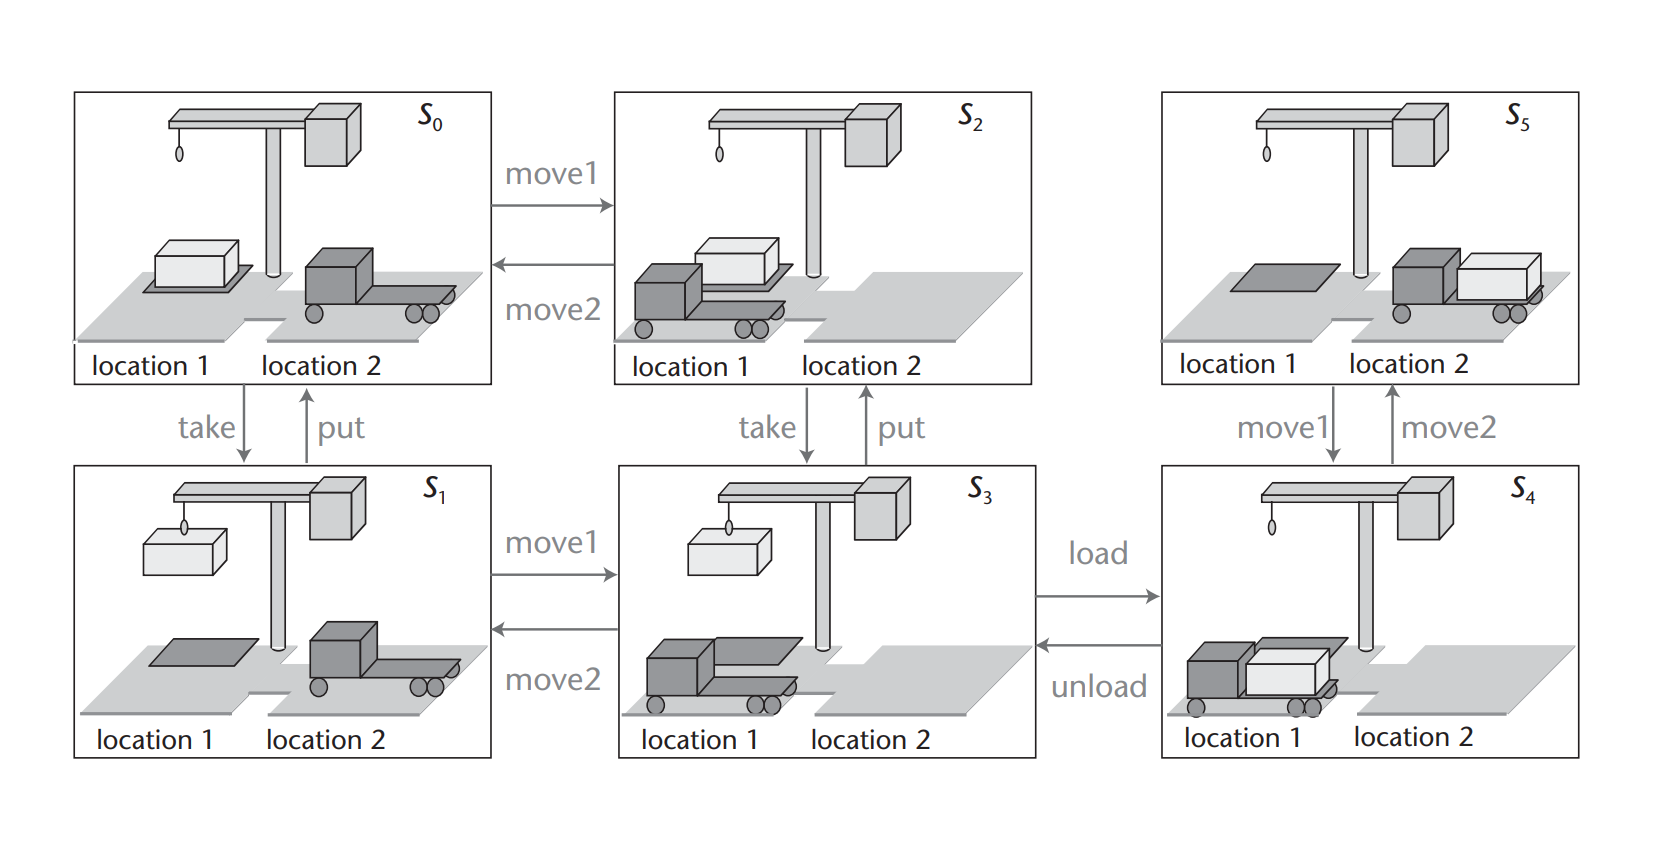
\includegraphics[width=1\linewidth]{figures/state-transition-example.png}
  \caption{A State-Transition System for a Simple Domain Involving a Crane and a
    Robot for Transporting Containers}
  \label{fig:state-transition-diagram}
\end{figure}

\section{Planners}
The planner's input is a \textit{planning problem}, which includes a description
of the system $\sum$, an initial situation and some objective. For example, in
figure \ref{fig:state-transition-diagram}, a planning problem $P$ might consist
of a description of $\sum$, the initial state $s_0$, and a single goal state
$s_5$.

The planner's output is a plan or policy that solves the planning problem. A
\textit{plan} is a sequence of actions such as

\begin{sspara}
$<$take, move1, load, move2$>$.
\end{sspara}

A \textit{policy} is a partial function from states into actions, such as

\begin{sspara}
$\{(s_0, take), (s_1, move1), (s_3, load), (s_4, move2)\}$.
\end{sspara}

The aforementioned plan and policy both solve the planning problem P. Either of
them, if executed starting at the initial state $s_0$, will take $\sum$ through
the sequence of states $\langle s1, s2, s3, s4, s5 \rangle$.

In general, the planner will produce actions that are described at an abstract
level. Hence it may be impossible to perform these actions without first
deciding some of the details. In many planning problems, some of these details
include what resources to use and what time to do the action.

\textit{What Resources to Use}. Exactly what is meant by a \textit{resource}
depends on how the problem is specified. For example, if $\sum$ contained more
than one robot, then one approach would be to require the robot's name as part
of the action (for example, \textsf{move1(robot)} and \textsf{move1(robot2))},
and another approach would be to consider the robot to be a resource whose
identity will be determined later.

\textit{What Time to Do the Action}. For example, in order to load the container
onto the robot, we might want to start moving the crane before the robot arrives
at \textsf{location1}, but we cannot complete the load operation until after the
robot has reached \textsf{location1} and has stopped moving.

In such cases, one approach is to have a separate program called a
\textit{scheduler} that sits in between the planner and the controller (see
figure \ref{fig:planner-diagram}c), whose purpose is to determine those
details. Another approach is to integrate the scheduling function directly into
the planner. The latter approach can substantially increase the complexity of
the planner, but on complex problems it can be much more efficient than having a
separate scheduler.

\section{Controllers}

The \textit{controller}'s input consists of plans (or schedules, if the system
includes a scheduler) and observations about the current state of the system.
The controller's output consists of actions to be performed in the
state-transition system.

In figure \ref{fig:planner-diagram}, notice that the controller is
\textit{online}. As it performs its actions, it receives \textit{observations},
each observation being a collection of sensor inputs giving information about
$\sum$'s current state. The observations can be modeled as an observation
function $\eta : S \rightarrow O$ that maps $S$ into some discrete set of
possible observations. Thus, the input to the controller is the observation $o =
\eta(s)$, where $s$ is the current state.

If $\eta$ is a one-to-one function, then from each observation $o$ we can deduce
exactly what state $\sum$ is in. In this case we say that the observations
provide \textit{complete} information. For example, in figure
\ref{fig:state-transition-diagram}, if there were a collection of sensors that
always provided the exact locations of the robot and the container, then this
sensor would provide complete information—or, at least, complete information for
the level of abstraction used in the figure.

If $\eta$ is not a one-to-one function, then the best we can deduce from an
observation $o$ is that $\sum$ is in one of the states in the set $\eta_{-1}(o)
\subseteq S$, and in this case we say that the observations provide
\textit{incomplete} information about $\sum$’s current state. For example, in
figure \ref{fig:state-transition-diagram}, if we had a sensor that told us the
location of the robot but not the location of the container, this sensor would
provide incomplete information.

\section{Assumptions in Classical Planning}
\label{appendix:assumptions}
\cite{Nau2007} also describes a set of assumptions that classical planners make
about the domain they will work on:

\paragraph*{\textit{Assumption A0 (Finite $\sum$).}} The system $\sum$ has a
finite set of states.

\paragraph*{\textit{Assumption A1 (Fully Observable $\sum$).}} The system $\sum$
is \textit{fully observable}, that is, one has complete knowledge about the
state of $\sum$; in this case the observation function $\eta$ is the identity
function.

\paragraph*{\textit{Assumption A2 (Deterministic $\sum$).}} The system $\sum$ is
\textit{deterministic}, that is, for every state $s$ and event or action $u$,
$|\gamma(s, u)| \leq 1$. If an action is applicable to a state, its application
brings a deterministic system to a single other state. Similarly for the
occurrence of a possible event.

\paragraph*{\textit{Assumption A3 (Static $\sum$).}} The system $\sum$ is
\textit{static}, that is, the set of events $E$ is empty. $\sum$ has no internal
dynamics; it stays in the same state until the controller applies some action.

\paragraph*{\textit{Assumption A4 (Attainment Goals).}} The only kind of goal is
an \textit{attainment goal}, which is specified as an explicit goal state or a
set of goal states $S_g$. The objective is to find any sequence of state
transitions that ends at one of the goal states. This assumption excludes, for
example, states to be avoided, constraints on state trajectories, and utility
functions.

\paragraph*{\textit{Assumption A5 (Sequential Plans).}} A solution plan to a
planning problem is a linearly ordered finite sequence of actions.

\paragraph*{\textit{Assumption A6 (Implicit Time).}} Actions and events have no
duration, they are instantaneous state transitions. This assumption is embedded
in the state-transition model, which does not represent time explicitly.

\paragraph*{\textit{Assumption A7 (Off-line Planning).}} The planner is not
concerned with any change that may occur in $\sum$ \textit{while} it is
planning; it plans for the given initial and goal states regardless of the
current dynamics, if any.

%%% Local Variables:
%%% mode: latex
%%% TeX-master: "../diss"
%%% End: